\documentclass[12pt]{article}
\usepackage[utf8]{inputenc}
\usepackage[spanish,es-tabla]{babel} % Opción spanish para traducir al español y es-tabla para que las tablas digan "Tabla" en vez de "Table".
\usepackage{geometry}
\usepackage{geometry}
\usepackage{listings}
\usepackage{color}
\usepackage{graphicx}
\usepackage{titlesec}
\usepackage{float}
\usepackage{amsmath}
\usepackage{hyperref}


% Configuración para el formato de los bloques de código
\definecolor{codegreen}{rgb}{0,0.6,0}
\definecolor{codegray}{rgb}{0.5,0.5,0.5}
\definecolor{codepurple}{rgb}{0.58,0,0.82}
\definecolor{backcolour}{rgb}{0.95,0.95,0.92}

\lstdefinestyle{mystyle}{
    backgroundcolor=\color{backcolour},   
    commentstyle=\color{codegreen},
    keywordstyle=\color{magenta},
    numberstyle=\tiny\color{codegray},
    stringstyle=\color{codepurple},
    basicstyle=\ttfamily\small,
    breakatwhitespace=false,         
    breaklines=true,                 
    captionpos=b,                    
    keepspaces=true,                 
    numbers=left,                    
    numbersep=5pt,                  
    showspaces=false,                
    showstringspaces=false,
    showtabs=false,                  
    tabsize=2
}

\lstset{style=mystyle}

% Configuración de la geometría de las páginas
\geometry{a4paper, top=3cm, bottom=2cm, left=3cm, right=3cm}

\begin{document}

% Portada
\begin{titlepage}
    \centering
    \vspace*{2cm}
    
    % Nombre de la Universidad
    {\Large\bfseries Universidad Tecnológica De Pereira\par}
    \vspace{1.5cm}
    
    % Facultad o Departamento (opcional)
    {\large Facultad de Ingeniería\par}
    \vspace{2cm}
    
    % Título del trabajo
    {\huge\bfseries Simulación de Péndulo Doble\par}
    \vspace{2cm}
    
    % Nombre del autor
    {\Large\itshape Jose Felipe Duarte Coronado\par}
    \vspace{1cm}
    
    % Nombre del profesor
    {\Large Profesor: Dr. Andrés Felipe Galvis\par}
    \vspace{2cm}
    
    % Lugar para agregar una imagen (opcional)
    % Descomenta las siguientes líneas si deseas añadir una imagen:
    
\includegraphics[width=0.5\textwidth]{Logo_U.T.P.png}
     \vspace{2cm}
    
    % Fecha
    {\large\today\par}
    \vfill
    
    % Nota sobre LaTeX
    {\footnotesize Documento generado con \LaTeX\par}
\end{titlepage}


\tableofcontents
\newpage

\section{Introducción}
El péndulo doble es un sistema mecánico que consiste en dos péndulos acoplados. Es un sistema fascinante debido a su naturaleza caótica, es decir, pequeñas variaciones en las condiciones iniciales pueden llevar a trayectorias notablemente diferentes. El objetivo de este informe es modelar y simular el comportamiento de un péndulo doble utilizando código de MATLAB. Además, se busca conectar las ecuaciones matemáticas que describen el sistema con su implementación en código para mostrar cómo la programación puede servir como una potente herramienta para entender sistemas físicos complejos.

\section{Teoría y Modelamiento Matemático}
Las ecuaciones de movimiento que rigen el comportamiento del péndulo doble pueden derivarse usando la dinámica de Lagrange. El sistema está constituido por dos péndulos acoplados con masas \(m_1\) y \(m_2\) y longitudes \(l_1\) y \(l_2\).

Las ecuaciones de movimiento son las siguientes:

\[
\begin{aligned}
\frac{d\theta_1}{dt} &= \omega_1 \\
\frac{d\theta_2}{dt} &= \omega_2 \\
\frac{d\omega_1}{dt} &= \frac{-g(2m_1 + m_2)\sin(\theta_1) - m_2g \sin(\theta_1 - 2\theta_2) - 2\sin(\theta_1 - \theta_2)m_2(\omega_2^2 l_2 + \omega_1^2 l_1 \cos(\theta_1 - \theta_2))}{l_1 (2m_1 + m_2 - m_2\cos(2\theta_1 - 2\theta_2))} \\
\frac{d\omega_2}{dt} &= \frac{2\sin(\theta_1 - \theta_2)(\omega_1^2 l_1 (m_1 + m_2) + g (m_1 + m_2) \cos(\theta_1) + \omega_2^2 l_2 m_2 \cos(\theta_1 - \theta_2))}{l_2 (2m_1 + m_2 - m_2\cos(2\theta_1 - 2\theta_2))}
\end{aligned}
\]

Donde \( \theta_1 \) y \( \theta_2 \) son los ángulos de los péndulos, y \( \omega_1 \) y \( \omega_2 \) son sus velocidades angulares respectivas. \( g \) es la aceleración debida a la gravedad.
 son las velocidades angulares respectivas.
\section{Código de la Simulación}

\subsection{Función principal: \texttt{double\_pendulum\_simulation}}
\begin{lstlisting}[language=Matlab]
function double_pendulum_simulation()
    % Función principal para simular un péndulo doble

    % Condiciones iniciales:
    % theta1 y theta2 son los ángulos iniciales (en radianes) de los péndulos 1 y 2, respectivamente.
    % omega1 y omega2 son las velocidades angulares iniciales (en rad/s) de los péndulos 1 y 2, respectivamente.
    y0 = [pi/2, 0.5, pi, 0.5];

    % Parámetros del péndulo:
    % m1 y m2 son las masas de los péndulos 1 y 2, respectivamente.
    % l1 y l2 son las longitudes de los péndulos 1 y 2, respectivamente.
    % g es la aceleración debida a la gravedad.
    p = [1, 1, 1, 1, 9.81];

    % Tiempo de simulación:
    % tspan es un vector que contiene los puntos de tiempo para los cuales se calcularán las soluciones.
    tspan = linspace(0, 20, 1000);

    % Resolver las ecuaciones diferenciales usando lsode (solver de Octave para ODEs)
    % Aquí usamos una función anónima para pasar los parámetros adicionales p a pendulumODE
    y = lsode(@(y, t) pendulumODE(y, t, p), y0, tspan);

    % Llamar a la función para animar el péndulo doble
    animate_pendulum(tspan, y, p);
end

\end{lstlisting}

Esta función sirve como punto de entrada para la simulación del péndulo doble. Se definen las condiciones iniciales para los ángulos \(\theta_1\) y \(\theta_2\) y las velocidades angulares \(\omega_1\) y \(\omega_2\) en el vector \(y0\). Los parámetros físicos del sistema, como las masas \(m_1\) y \(m_2\), las longitudes \(l_1\) y \(l_2\), y la aceleración debida a la gravedad \(g\), se definen en el vector \(p\).

Se utiliza la función `lsode` para resolver las ecuaciones diferenciales ordinarias (ODEs) que describen el sistema, llamando a la función `pendulumODE`.

\subsection{Función del sistema de ecuaciones: \texttt{pendulumODE}}
\begin{lstlisting}[language=Matlab]
function dy = pendulumODE(y, t, p)
    % Extraer parámetros del péndulo del vector p
    m1 = p(1); % Masa del primer péndulo
    m2 = p(2); % Masa del segundo péndulo
    l1 = p(3); % Longitud del primer péndulo
    l2 = p(4); % Longitud del segundo péndulo
    g = p(5);  % Aceleración debida a la gravedad

    % Calcular la diferencia entre los ángulos del primer y segundo péndulo
    delta = y(3) - y(1);

    % Calcular el cuadrado de las velocidades angulares
    omega1_squared = y(2)^2;
    omega2_squared = y(4)^2;

    % Calcular los denominadores que aparecerán en las ecuaciones diferenciales
    den1 = (m1+m2) * l1 - m2 * l1 * cos(delta)^2;
    den2 = (l2/l1) * den1;

    % Verificar si los denominadores son cercanos a cero para evitar división por cero
    if abs(den1) < 1e-6
        den1 = 1e-6;
    end
    if abs(den2) < 1e-6
        den2 = 1e-6;
    end

    % Inicializar el vector dy como un vector columna de ceros
    dy = zeros(4,1);

    % Calcular las derivadas para las ecuaciones de movimiento del péndulo doble
    dy(1) = y(2);  % Velocidad angular del primer péndulo
    dy(2) = ((m2 * l2 * omega2_squared * sin(delta) * cos(delta) ...
        + m2 * g * sin(y(3)) * cos(delta) ...
        + m2 * l2 * omega2_squared * sin(delta) ...
        - (m1 + m2) * g * sin(y(1))) ...
        / den1 );
    dy(3) = y(4);  % Velocidad angular del segundo péndulo
    dy(4) = ((- l1 / l2) * omega1_squared * sin(delta) * cos(delta) ...
        + (m1 + m2) * g * sin(y(1)) * cos(delta) ...
        - (m1 + m2) * l1 * omega1_squared * sin(delta) ...
        - (m1 + m2) * g * sin(y(3))) ...
        / den2 );
end

\end{lstlisting}

Esta función implementa las ecuaciones de movimiento del péndulo doble. Los ángulos y las velocidades angulares se pasan en el vector \(y\), mientras que el tiempo \(t\) y los parámetros \(p\) se pasan como argumentos adicionales.

Se calculan los denominadores \(den1\) y \(den2\) para las ecuaciones del sistema. Estos valores se usan para evitar divisiones por cero o valores cercanos a cero. Finalmente, se devuelve un vector \(dy\) que contiene las derivadas de los ángulos y las velocidades angulares, que `lsode` utiliza para resolver las ecuaciones de movimiento.

\subsection{Función de animación: \texttt{animate\_pendulum}}
\begin{lstlisting}[language=Matlab]
function animate_pendulum(t, y, p)
    % Función para animar el péndulo doble
    
    % Extraer las longitudes l1 y l2 de los péndulos del vector de parámetros p
    l1 = p(3); l2 = p(4);
    
    % Inicializar la figura y los trazados
    figure(1);
    ground = plot([-2*l1, 2*l1], [0, 0], 'r'); % Dibujo del suelo
    hold on;
    
    % Inicializar la primera y segunda línea del péndulo con sus respectivas masas
    pendulum1 = line([0, l1*sin(y(1,1))], [0, -l1*cos(y(1,1))], 'LineWidth', 2, 'Marker', 'o', 'MarkerSize', 10);
    pendulum2 = line([l1*sin(y(1,1)), l1*sin(y(1,1)) + l2*sin(y(1,3))], [-l1*cos(y(1,1)), -l1*cos(y(1,1)) - l2*cos(y(1,3))], 'LineWidth', 2, 'Marker', 'o', 'MarkerSize', 10);
    
    % Inicializar arreglos para almacenar las posiciones de los péndulos con el fin de trazar su trayectoria
    trace1_x = [];
    trace1_y = [];
    trace2_x = [];
    trace2_y = [];
    
    % Configurar los ejes de la gráfica
    axis equal;
    axis([-2*l1, 2*l1, -2*l1, 2*l1]);
    grid on;
    
    % Calcular el paso de tiempo entre los puntos de datos
    dt = t(2) - t(1);
    
    % Bucle para actualizar la animación en cada paso de tiempo
    for k = 1:length(t)
        % Actualizar las posiciones del péndulo usando la función set
        set(pendulum1, 'XData', [0, l1*sin(y(k,1))], 'YData', [0, -l1*cos(y(k,1))]);
        set(pendulum2, 'XData', [l1*sin(y(k,1)), l1*sin(y(k,1)) + l2*sin(y(k,3))], 'YData', [-l1*cos(y(k,1)), -l1*cos(y(k,1)) - l2*cos(y(k,3))]);
        
        % Añadir las posiciones actuales para el trazado de las trayectorias
        trace1_x = [trace1_x, l1*sin(y(k,1))];
        trace1_y = [trace1_y, -l1*cos(y(k,1))];
        trace2_x = [trace2_x, l1*sin(y(k,1)) + l2*sin(y(k,3))];
        trace2_y = [trace2_y, -l1*cos(y(k,1)) - l2*cos(y(k,3))];
        
        % Dibujar las trayectorias
        plot(trace1_x, trace1_y, 'g-');
        plot(trace2_x, trace2_y, 'b-');
        
        % Actualizar el título para mostrar el tiempo actual
        title(sprintf('Tiempo: %.2f s', t(k)));
        
        % Pausar la animación para hacerla coincide con la resolución de la solución ODE
        pause(dt);
    end
    hold off;
end

\end{lstlisting}

Esta función anima el péndulo doble usando los resultados de la simulación. Se grafican las posiciones de los péndulos en tiempo real, mostrando también sus trayectorias. Los ángulos y las velocidades angulares se toman del argumento \(y\) y se usan para calcular las posiciones \(x\) e \(y\) de cada péndulo en cada instante de tiempo \(t\).

Se utilizan las funciones `set` y `plot` de Matlab para actualizar la posición de los péndulos y trazar sus trayectorias a medida que evoluciona el sistema.



\section{Resultados y Animación}

La animación generada proporciona una representación visual del comportamiento dinámico del péndulo doble a lo largo del tiempo. Además, se han generado gráficos estáticos que muestran la evolución de los ángulos \(\theta_1\) y \(\theta_2\), así como las velocidades angulares \(\omega_1\) y \(\omega_2\), con respecto al tiempo (ver Figura \ref{fig:evolucion}).

\begin{figure}[H]
\centering
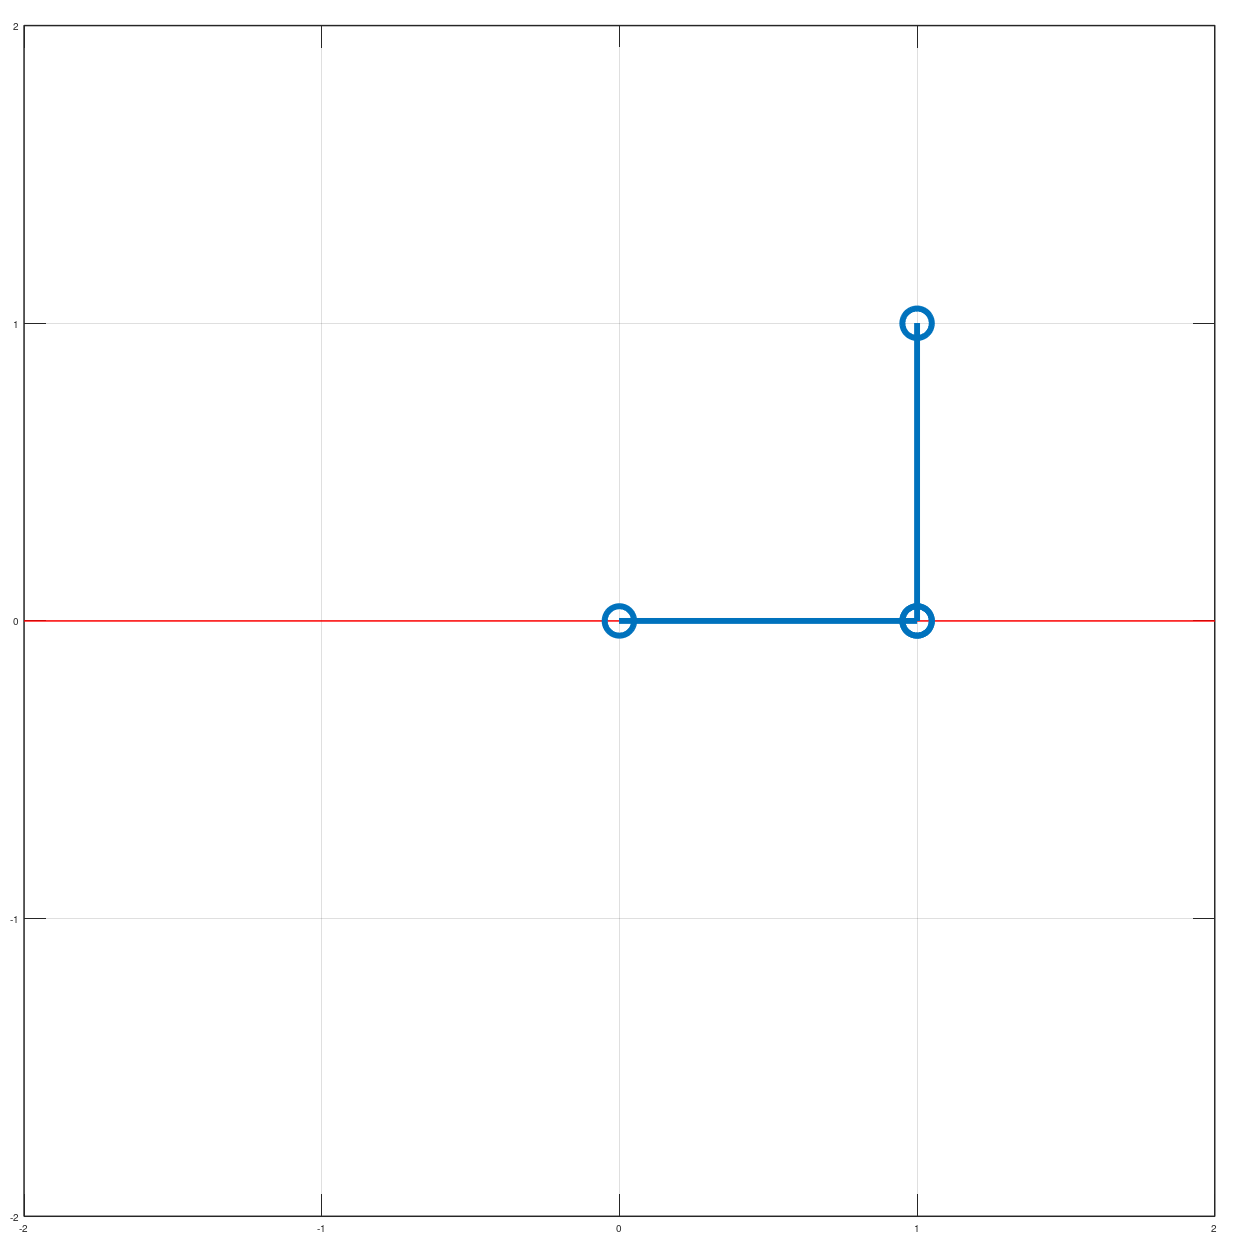
\includegraphics[width=0.5\textwidth]{evolucion.png}
\caption{Evolución de los ángulos y velocidades angulares con respecto al tiempo.}
\label{fig:evolucion}
\end{figure}

Las trayectorias trazadas por los extremos de los péndulos también se han visualizado en un espacio bidimensional, lo que demuestra el comportamiento caótico del sistema (ver Figura \ref{fig:trayectoria}).

\begin{figure}[H]
\centering
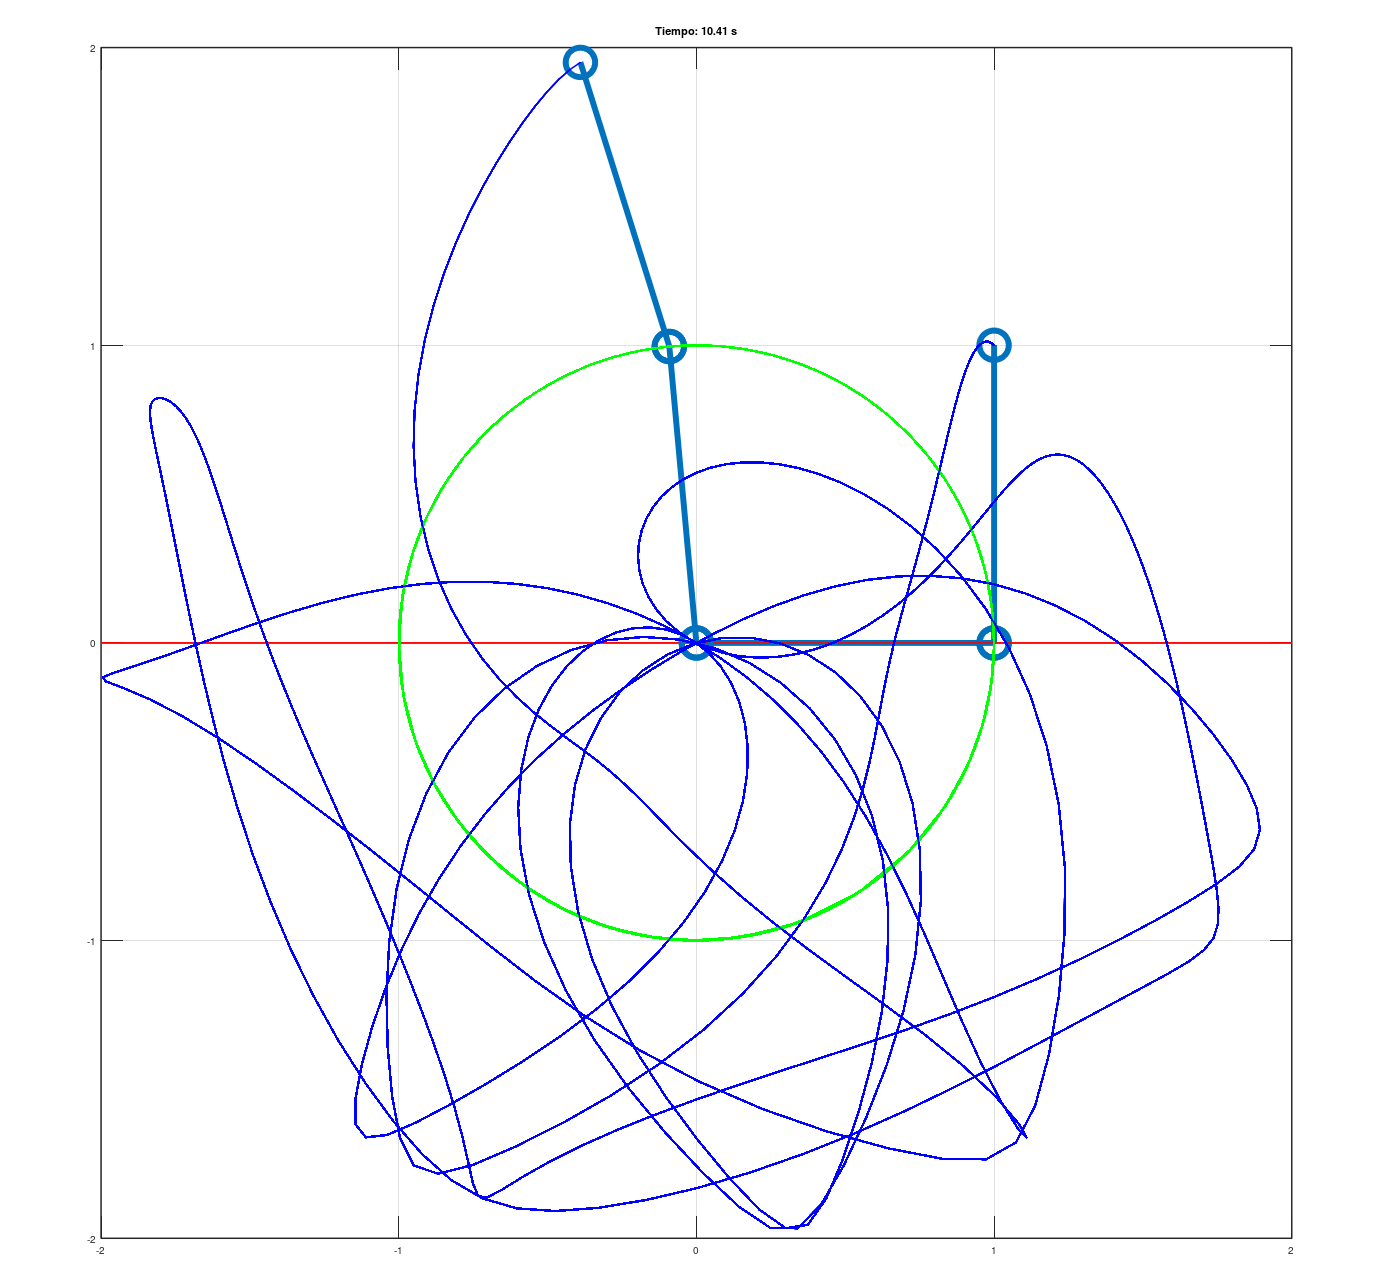
\includegraphics[width=0.5\textwidth]{trayectoria.png}
\caption{Trayectorias del extremo del péndulo doble.}
\label{fig:trayectoria}
\end{figure}

Estas visualizaciones proporcionan una comprensión profunda de cómo pequeñas variaciones en las condiciones iniciales pueden llevar a comportamientos drásticamente diferentes, una característica inherente de los sistemas caóticos.


\section{Conclusión}

Este proyecto ha proporcionado una oportunidad valiosa para explorar la dinámica compleja del péndulo doble, un sistema mecánico que exhibe comportamiento caótico. A través de la modelación matemática y la simulación computacional, hemos podido visualizar y entender cómo las condiciones iniciales y los parámetros del sistema afectan su comportamiento dinámico.

La animación y los gráficos generados brindan una representación visual clara del movimiento del péndulo doble, y demuestran cómo la programación puede ser una herramienta poderosa para explorar y entender sistemas físicos complejos. Además, este trabajo resalta la importancia de las visualizaciones en la comunicación efectiva de conceptos dinámicos complejos.

Aunque se logró una comprensión significativa del sistema, también se encontraron desafíos, especialmente en la gestión de la precisión numérica y la estabilidad de la simulación en presencia de comportamiento caótico. Futuras extensiones de este trabajo podrían incluir la exploración de diferentes métodos numéricos para mejorar la precisión de la simulación, o la incorporación de controladores para estabilizar el movimiento del péndulo doble.



\section{Anexos}

El código fuente completo para la simulación está disponible en GitHub en el siguiente enlace:
\begin{center}
    \url{hhttps://github.com/josefdc/Simulacion-Doble-Pendulo}
\end{center}

El video con las simulaciones puede ser encontrado en:
\begin{center}
    \url{https://youtu.be/ltXBXmy90iI}
\end{center}


\begin{thebibliography}{9}

\bibitem{researchgate1}
\textit{Simulation of Double Pendulum},
ResearchGate,
\url{https://www.researchgate.net}[5†source].

\bibitem{mathworks}
\textit{Modeling Mechanical Systems: The Double Pendulum},
Mathworks,
\url{https://blogs.mathworks.com}[6†source].

\bibitem{researchgate2}
Mehmet Han İnyayla, Aydın Adnan Menderes,
\textit{Modeling and Simulation for the Double Pendulum (2DOF) Using Lagrange's Equations in MATLAB},
ResearchGate, February 2023,
\url{https://www.researchgate.net}[7†source].

\bibitem{acmsigsim}
Randolph J. Taylor,
\textit{Simulation of double pendulum motion},
ACM SIGSIM Simulation Digest, Volume 10, Issue 1-2, Fall-Winter 1978-1979, pp 20–25,
\url{https://doi.org/10.1145/1102786.1102789}[8†source].

\bibitem{ieeexplore}
\textit{The Mathematical Modeling of a Double-Pendulum System as a Physical Model of Flexible Arm Robot},
IEEE Xplore,
\url{https://ieeexplore.ieee.org}[9†source].

\end{thebibliography}

\end{document}
